\section{Ordenación elemental}
El problema de ordenar un conjunto de elementos es uno de los problemas más estudiados en la historia de la computación. Existen numerosos algoritmos para resolver este problema, cada uno con sus propias características y desventajas. En esta sección estudiaremos el algoritmo de ordenación más sencillo (pero no el más rápido), cuyo procedimiento es el siguiente:

\begin{enumerate}
    \item \textbf{Selecciona} el menor de todos, lo intercambia con el elemento que se encuentra en la primera posición.
    \item \textbf{Selecciona} el menor de los restantes, lo intercambia con el elemento que se encuentra en la segunda posición. 
    \item \textbf{Selecciona} el menor de los restantes, lo intercambia con el elemento que se encuentra en la tercera posición. 
    \item ... y así sucesivamente hasta que el conjunto esté ordenado.  
\end{enumerate}

\subsection{Recurso gráfico}
Para ilustrar el funcionamiento del algoritmo de ordenación por selección, se ha desarrollado un recurso gráfico que permite visualizar el estado del conjunto en cada iteración. Supongamos que se tiene la lista:
\begin{equation*}
    [ \ 9,3,1,3,5,27 \ ]
\end{equation*}
y lo que se busca es aplicar el algoritmo de ordenación por selección.

\begin{figure}[H]
    \centering
    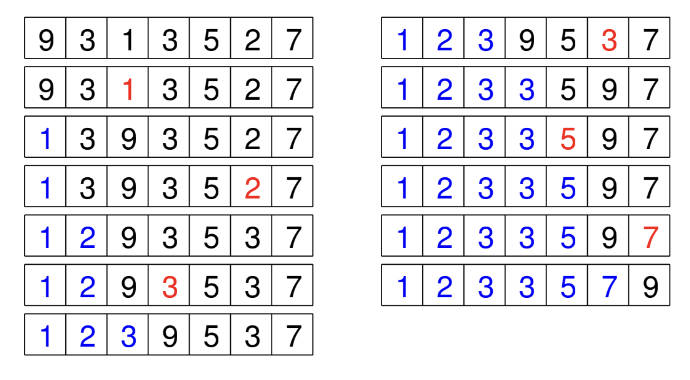
\includegraphics[scale=0.5]{./Images/oedef.png}
    \caption{Paso a paso de la ordenación por selección.}
\end{figure}


\subsection{Código}

\begin{pascallike}
proc selection_sort (in/out a: array[1..n] of T)
    var minp: nat
    for i := 1 to n do
        minp := min_pos_from(a, i)
        swap(a, i, minp) 
    od
end proc

fun min_pos_from (a: array[1..n] of T, i: nat) ret minp: nat
    minp := i
    for j:= i+1 to n do 
        if a[j] < a[minp] then 
            minp:= j 
        fi
    od
end fun

proc swap (in/out a: array[1..n] of T, in i, j: nat)
    var temp: T
    temp := a[i]
    a[i] := a[j]
    a[j] := temp
end proc
\end{pascallike}

Para el algoritmo de ordenación por selección, se ha desarrollado un procedimiento \texttt{selection\_sort} que recibe un arreglo de tamaño $n$ y lo ordena. El procedimiento \texttt{selection\_sort} utiliza dos funciones auxiliares: \texttt{min\_pos\_from} y \texttt{swap}. La función \texttt{min\_pos\_from} recibe un arreglo y una posición, y retorna la posición del menor elemento a partir de la posición dada. La función \texttt{swap} recibe un arreglo y dos posiciones, e intercambia los elementos en dichas posiciones. Se pueden marcar las siguientes observaciones:

\begin{itemize}
    \item \texttt{selection\_sort} utiliza un ciclo \texttt{for} que recorre el arreglo desde la primera posición hasta la última. En cada iteración, se busca el menor elemento a partir de la posición actual y se intercambia con el elemento en la posición actual,
    \item se encuentra una llamada a la función \texttt{min\_pos\_from} que recibe el arreglo y la posición actual, y retorna la posición del menor elemento a partir de la posición actual,
    \item y se recibe tambien una llamada al procedimiento \texttt{swap} que recibe el arreglo y las posiciones actual y la posición del menor elemento, e intercambia los elementos en dichas posiciones,
    \item encontramos una \textbf{comparación} entre elementos de un arreglo, y una \textbf{asignación} de elementos de un arreglo,
    \item la operación que mas se repite es la comparación de elementos de un arreglo, y toda operación se repite a lo sumo de manera proporcional a esa,
    \item como la celda de un arreglo es constante, su costo no depende de cual es la celda o del tamaño del arreglo, por lo que el costo de la operación es constante.
\end{itemize}